\begin{frame}[allowframebreaks]{UMAP to the rescue!}
    \begin{itemize}
        \item UMAP is a replacement for t-SNE, designed to fulfill the same role in dimensionality reduction.
        \item It is conceptually very similar to t-SNE, but introduces several relevant (and somewhat technical) changes.
        \item In practice, UMAP offers several advantages:
        \begin{itemize}
            \item UMAP is significantly faster than t-SNE.
            \item It can preserve more global structure compared to t-SNE.\footnote{Preservation of global structure may depend on the dataset and parameter choices.}
            \item UMAP can operate directly on raw data without requiring PCA preprocessing.\footnote{Although PCA preprocessing can still be beneficial in some cases.}
            \item It allows new data points to be added to an existing projection, enabling incremental updates.
        \end{itemize}
    \end{itemize}
\end{frame}


\begin{frame}[allowframebreaks]{UMAP differences}
    \begin{itemize}
        \item Unlike t-SNE, which uses a single perplexity parameter, UMAP introduces two key parameters:
        \begin{itemize}
            \item \textbf{Number of Nearest Neighbours:} Specifies how many nearest neighbours are considered for each point. This is conceptually similar to perplexity in t-SNE and controls the balance between local and global structure in the embedding.
            \item \textbf{Minimum Distance:} Determines how closely UMAP packs points together in the low-dimensional space. Lower values allow points to be closer, resulting in more compact clusters, while higher values spread points apart.
        \end{itemize}
        \item The \textbf{nearest neighbours} parameter influences the trade-off between preserving local versus global structure in the data.
        \item The \textbf{minimum distance} parameter affects the density and compactness of clusters in the resulting visualization.
        \item Together, these parameters provide more flexibility and control over the embedding compared to t-SNE's single perplexity value.
    \end{itemize}

    \framebreak

    \textbf{Structure preservation} – mostly in the 2D projection scoring
    \vspace{1em}
    \begin{columns}
    \begin{column}{0.4\textwidth}
        \begin{figure}
            \centering
            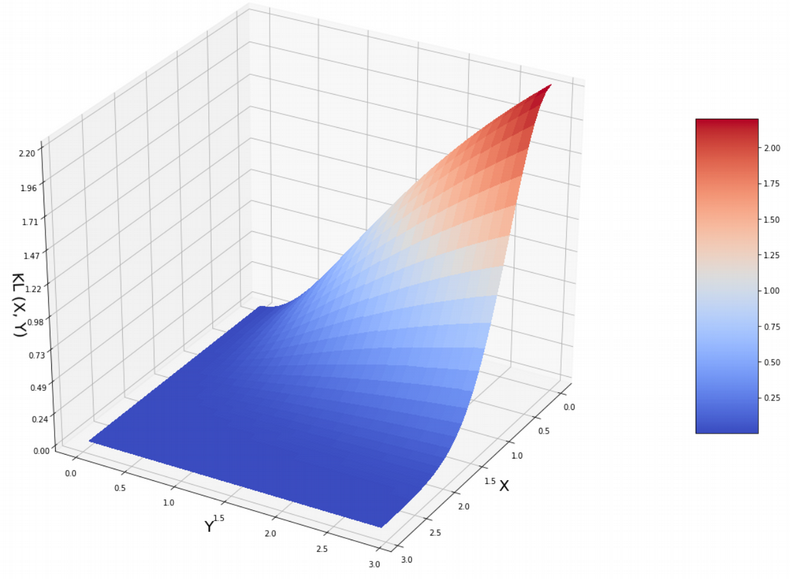
\includegraphics[width=1\textwidth,keepaspectratio]{images/dul/dim-reduce/slide_41_1_img.png}
            \caption{t-SNE}
        \end{figure}
    \end{column}
    \begin{column}{0.4\textwidth}
        \begin{figure}
            \centering
            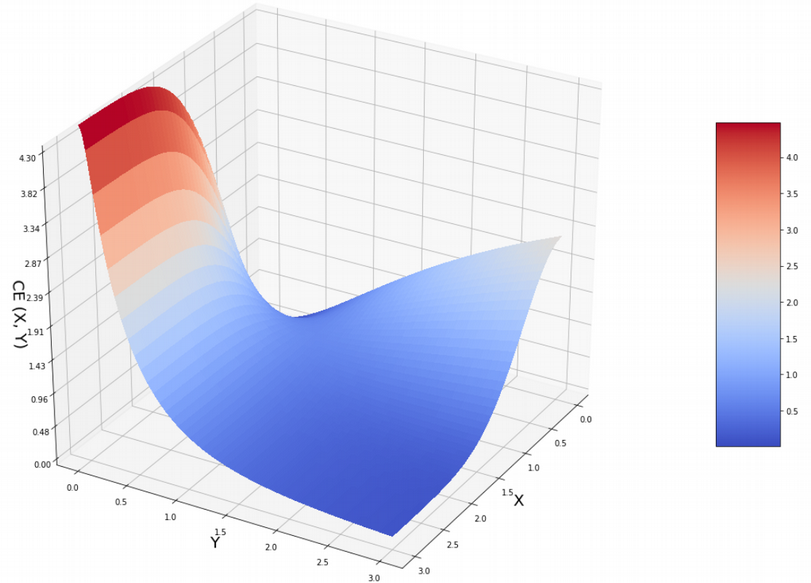
\includegraphics[width=1\textwidth,keepaspectratio]{images/dul/dim-reduce/slide_41_2_img.png}
            \caption{UMAP}
        \end{figure}
    \end{column}
    \begin{column}{0.22\textwidth}
        \begin{figure}
            \centering
            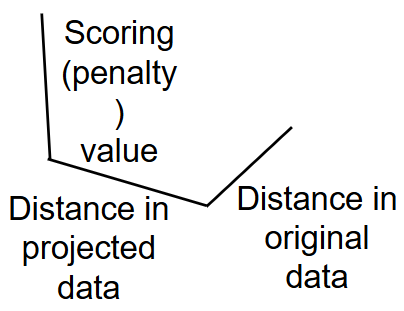
\includegraphics[width=1\textwidth,keepaspectratio]{images/dul/dim-reduce/slide_41_3_img.png}
        \end{figure}
    \end{column}
    \end{columns}
\end{frame}

\begin{frame}[allowframebreaks]{So UMAP is great then?}
    \begin{figure}
        \centering
        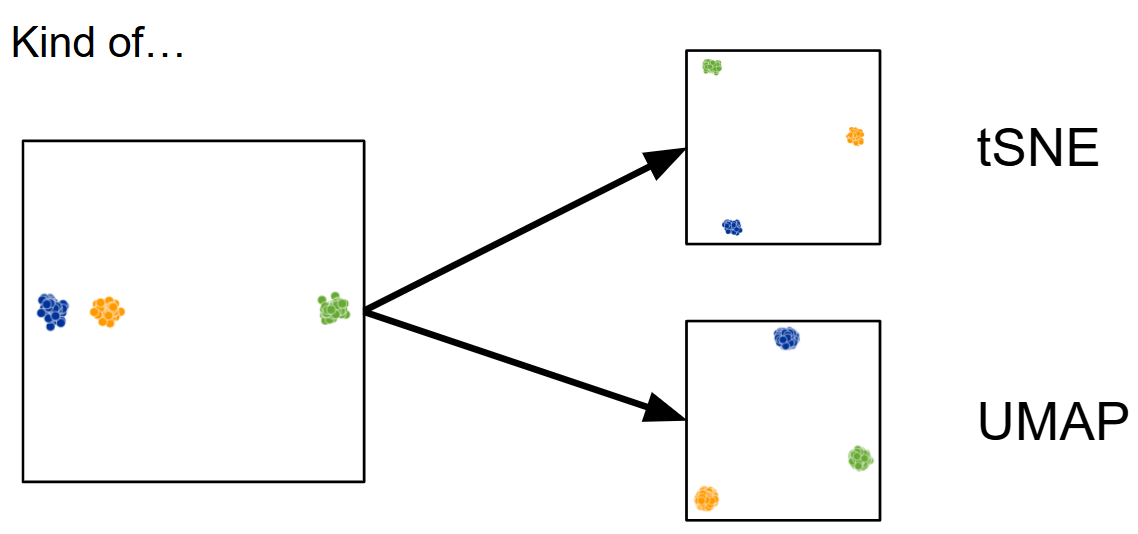
\includegraphics[width=1\textwidth,keepaspectratio]{images/dul/dim-reduce/slide_42_1_img.png}
    \end{figure}
\end{frame}

\begin{frame}[allowframebreaks]{So UMAP is all hype then?}
    \begin{figure}
        \centering
        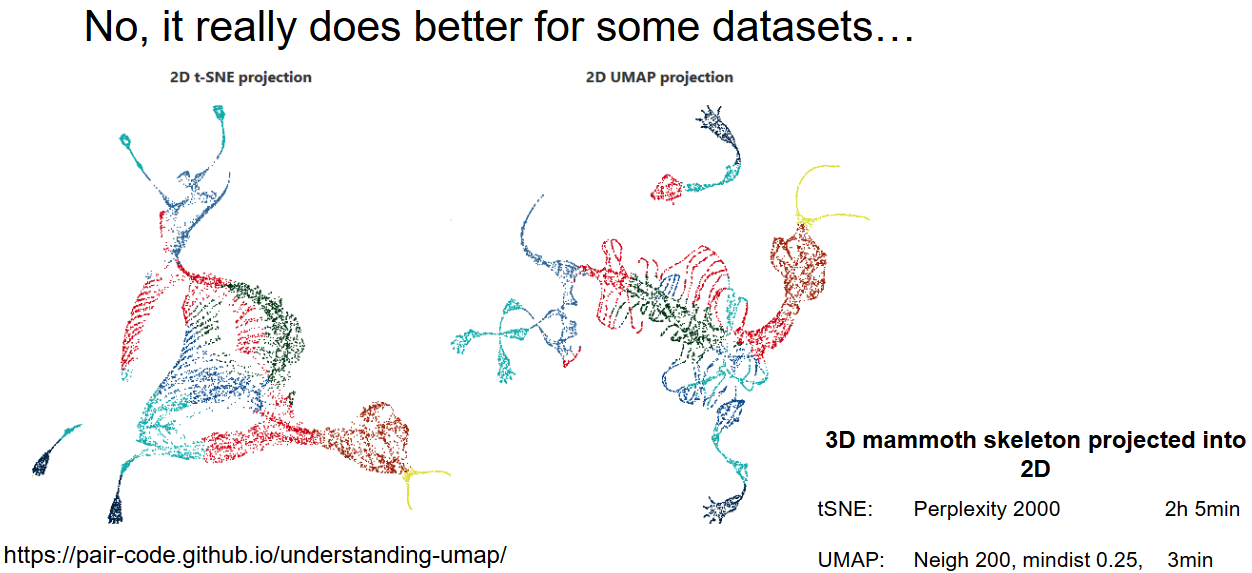
\includegraphics[width=1\textwidth,keepaspectratio]{images/dul/dim-reduce/slide_43_1_img.png}
    \end{figure}
\end{frame}


\begin{frame}[allowframebreaks]{Practical approach PCA + tSNE/UMAP}
    \begin{itemize}
        \item \textbf{Filter the data:}
        \begin{itemize}
            \item Remove poorly behaving cells to ensure data quality.
            \item Select only expressed genes for further analysis.
            \item Identify and retain variable genes to focus on informative features.
        \end{itemize}
        \item \textbf{Apply PCA (Principal Component Analysis):}
        \begin{itemize}
            \item Extract the most interesting and informative signals from the data.
            \item Select the top principal components (PCs) to reduce dimensionality, but do not reduce directly to 2 dimensions.
        \end{itemize}
        \item \textbf{Run t-SNE or UMAP:}
        \begin{itemize}
            \item Calculate distances between samples using the PCA projections.
            \item Scale these distances appropriately.
            \item Project the data into 2 dimensions for visualization using t-SNE or UMAP.
        \end{itemize}
    \end{itemize}
\end{frame}

\begin{frame}[allowframebreaks]{So PCA + UMAP is great then?}
    \begin{columns}
    \begin{column}{0.4\textwidth}
        \begin{itemize}
            \item Kind of\ldots{} as long as you only have one dataset.
            \begin{itemize}
                \item In 10X experiments, each library is considered a \textbf{batch}.
                \item Over time or distance, additional biases can be introduced.
                \item These biases make direct comparisons between datasets challenging.
                \item To enable meaningful comparisons, it is necessary to align the datasets and correct for batch effects.
            \end{itemize}
        \end{itemize}
    \end{column}
    \begin{column}{0.6\textwidth}
        \begin{figure}
            \centering
            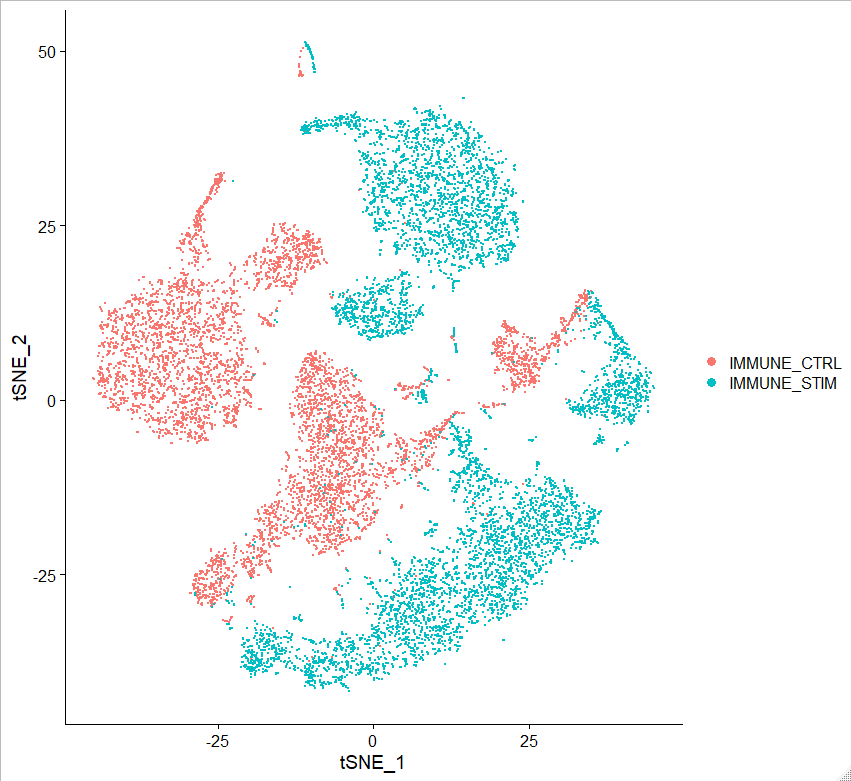
\includegraphics[width=1\textwidth,keepaspectratio]{images/dul/dim-reduce/slide_45_1_img.png}
            \caption{UMAP}
        \end{figure}
    \end{column}
    \end{columns}
\end{frame}